Method here, in past tense.

We reference like this using \verb|cleveref|: \cref{int:fig:example_a}, \cref{theo:eq:newton2}.

\subsection{Datasets}
    \comment{Here we describe how we construct and prepare the dataset. -\Carl}

    \subsubsection{MNIST}
        A simpler test for our neural networks is the MNIST benchmark dataset. It consists of 60 000 training images and 10 000 testing images. Each image consists $28 \times 28$ pixels depicting handwritten number between 0 and 9. As such, the images are to be classified to one of the 10 categories of digits.

    \subsubsection{CIFAR-10}
        Initially, we applied our the LWTA NNs on the CIFAR-10 benchmark dataset for image recognition. This dataset consists of 60 000 images with $32 \times 32$ coloured pixels with RGB values, amounting to 3072 features per image. The images are divided into 10 categories, depicting one of either aeroplanes, birds, cars, cats, deer, dogs, frogs, horses, ships or trucks (see \cref{met:fig:CIFAR10}).

        \begin{figure}[ht!]
            \centering
            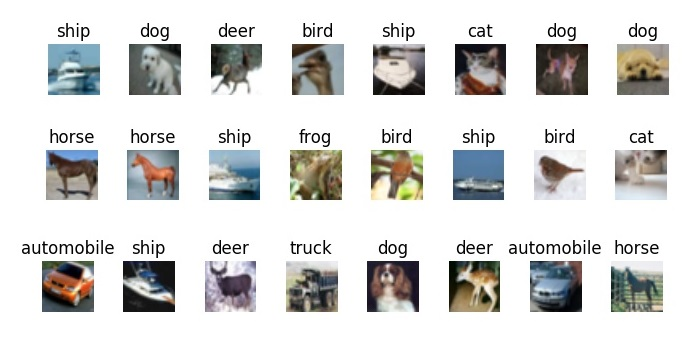
\includegraphics[width=\linewidth]{CIFAR10_examples.jpg}
            \caption{Examples of the images in the CIFAR10 dataset.}
            \label[fig]{met:fig:CIFAR10}
        \end{figure}

    \subsubsection{Premier League 2019 Season?}


    \subsubsection{Data Preparation}
        \comment{Describe preprocessing of data, i.e. scaling etc. -\Carl}
        \comment{Data splitting \Anna}
        To train and evaluate our models we implemented the relevant data and and as in our previous projects we split it in training data ($\sfrac{5}{6}$ of the data) and testing data ($\sfrac{1}{6}$ of the data) \citep{Project1}\citep{Project2}. When tuning the architecture, we further split the training data into a tuning set and a validation set used for monitoring overfitting, implementing early stopping with $p=5$. We used a split of $\sfrac{3}{4}$. See \cref{the:fig:illustration_data} for illustration of the data splitting. 

        \begin{figure}[]
            \centering
            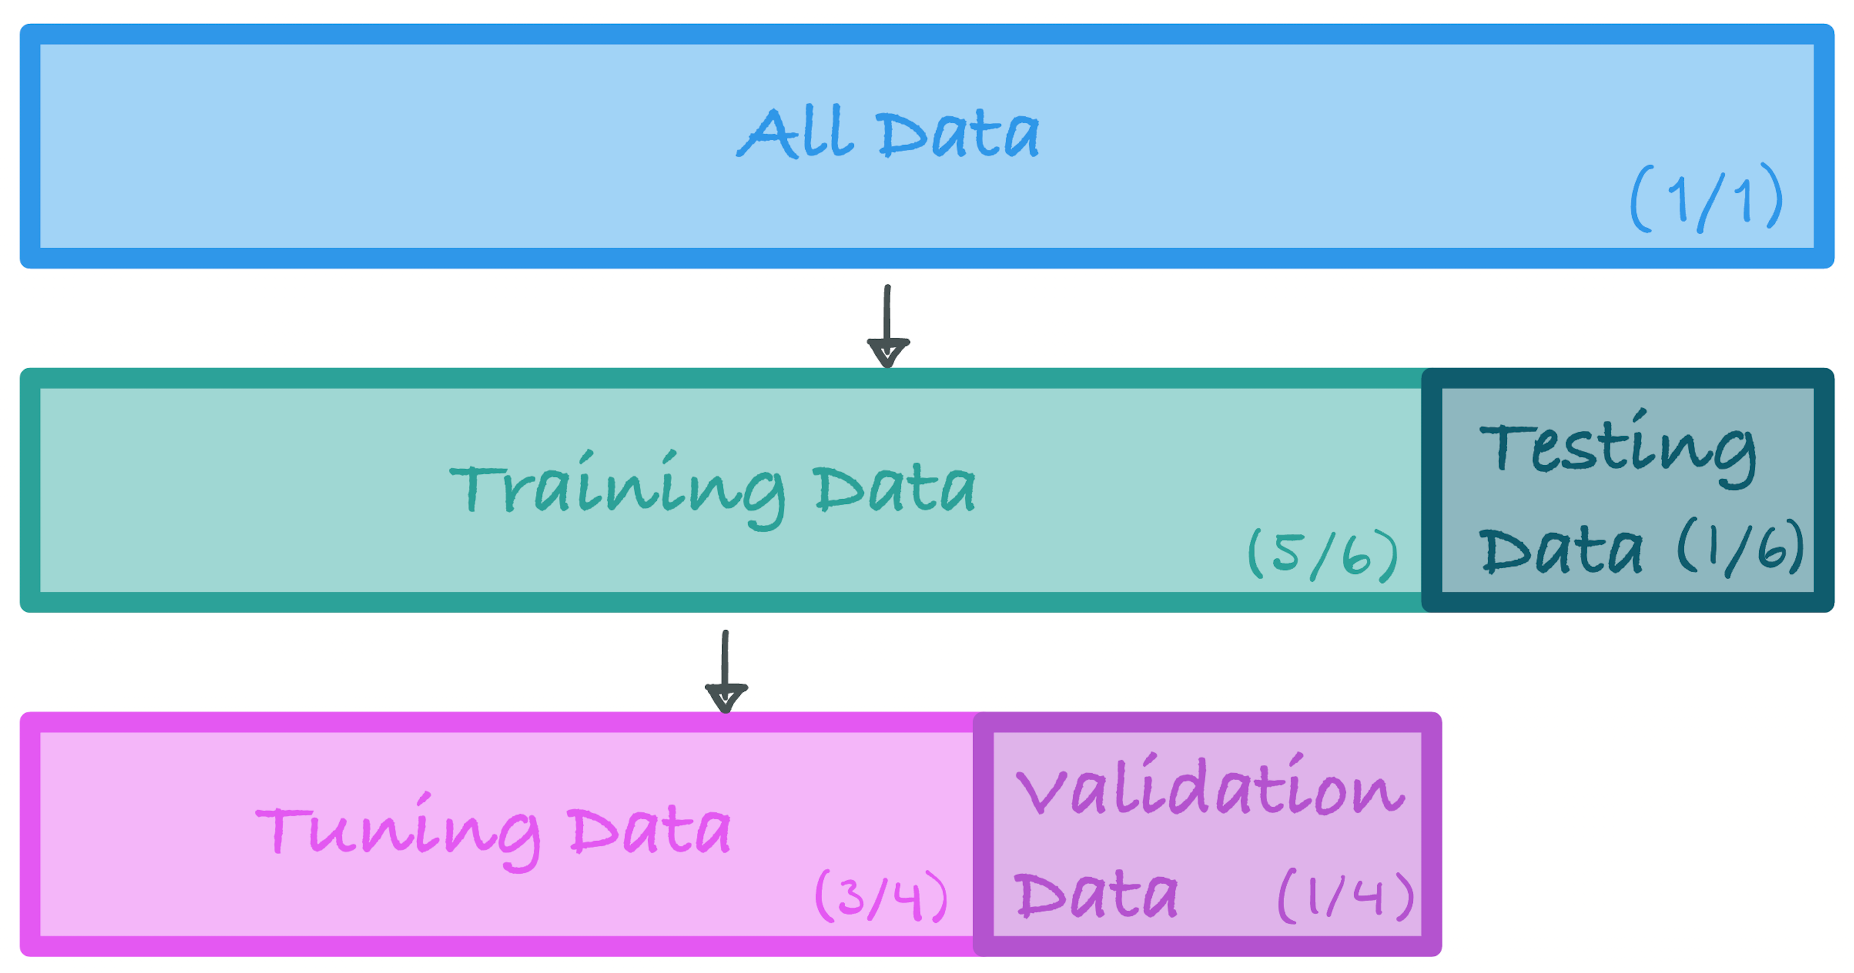
\includegraphics[width=.9\linewidth]{illustration_data.png}
            \caption{Illustration of data splitting.}
            \label[fig]{the:fig:illustration_data}
        \end{figure}

    \subsubsection{PCA}
        \comment{Could perhaps be part of data preparation \Anna}


\subsection{Neural Network training}

    \subsubsection{Initialisation of the Neural Network Weights}
        It is important to take care when initialising the weights and biases of a neural network to ensure fast convergence during training. We initialised the weights according to the He algorithm~\citep{He}. In our case it meant initialising the weights of node $i$ in layer $\ell$ by the distribution
        \begin{align}
            w^\ell_{ij} \distas \normal{0}{\sqrt{2/\hat{n}}},
        \end{align}
        where $\hat{n}$ is the number of inputs to the layer. The biases were all initialised to zero.

    \subsubsection{Optimisation Algorithm}
        When optimising the cost function of our problems we built on what we found in \citep{Project2}, using stochastic gradient descent with a batch size of 32. We used the Adam algorithm with hyperparameters $\beta_1 = 0.9$, $\beta_2 = 0.999$ and a learning rate $\eta = 0.001$. These hyperparameters were not tuned in any of our searches. The number of training epochs was decided with early stopping termination criterion. This means monitoring the loss of the network on a validation dataset after each epoch of training, and stopping the training if there is no improvement after a number of epochs $p$, called the \textit{patience}.

        All the datasets used pose classification problems with 3 or 10 categories. The cost function we used for optimisation was the standard categorical cross-entropy. Predicting $\vec{\tilde{y}}$ for the datapoints $\vec{y}$, with $n$ datapoints and $C$ categories, the categorical cross-entropy is given by
        \begin{align}
            \mathcal{L}(\tilde{y}) = \sum_{i=1}^n \sum_{c \in \mathrm{categories}} y_i \log\pclosed{y=c|\tilde{y}_i}
        \end{align}

        \comment{Discussion note: Early stopping prevents overfitting. -\Carl}

    \subsubsection{Regularisation}
        \comment{Write about L2-regularisation. -\Carl}

        A problem that can occur in LWTA layers is when the weights of one node becomes much larger than those of the other nodes in the group, resulting in training of just this single node. A common technique to combat this is to add a dropout layer before and/or after the LWTA layer. The dropout layer randomly sets elements in its input vector to zero, according to a dropout rate, before passing it on to the next layer. This means that the nodes in a group cannot solely lean on one specific node, and forces pathways in the network to not learn specific trends `too much'. As such, it prevents overfitting, and can be seen as a regularisation method. The dropout layers are only active during training, and do not drop any activations at inference time. The effect of dropout on a LWTA network is illustrated in \cref{met:fig:dropout_network}.

        \begin{figure}
            \centering
            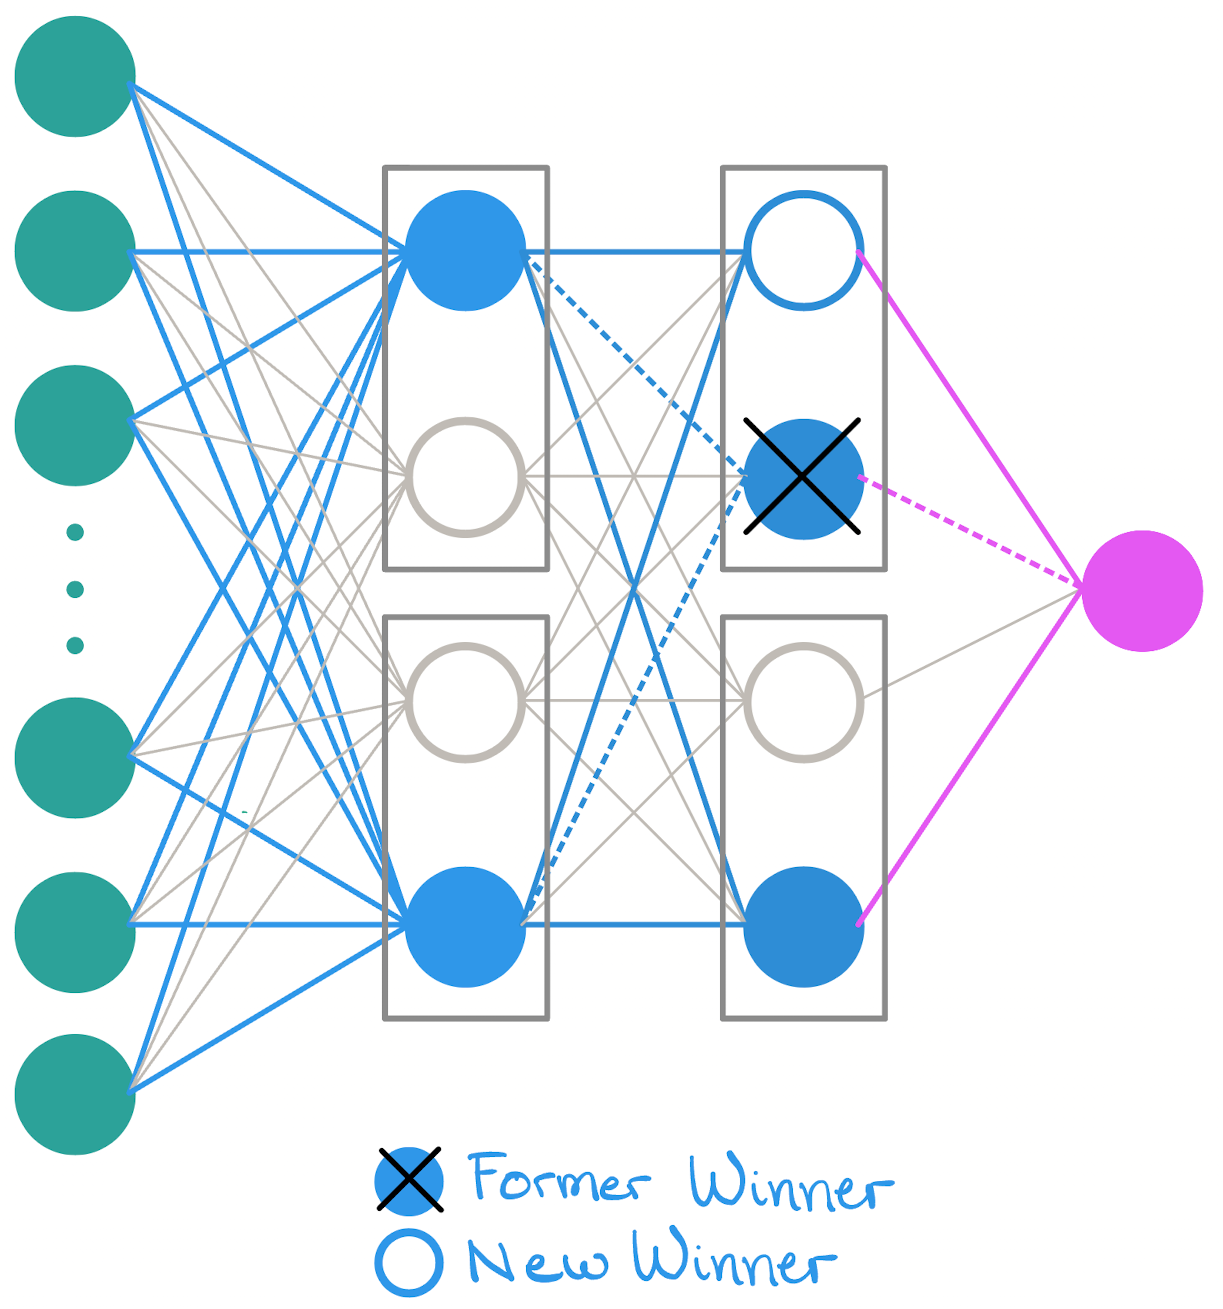
\includegraphics[width=\linewidth]{figs/illustration_dropout.png}
            \caption{An illustration channel-out neural network with a dropout added to the second channel-out layer.}
            \label[fig]{met:fig:dropout_network}
        \end{figure}

        We added dropout to our networks to see whether the performance was improved. \comment{Write more on this when it has been done.}


\subsection{Architecture tuning}
    To see what kind of network architectures were interesting and useful when applying to the datasets at hand, we tuned the architecture using the \textit{hyperband} search algorithm \citep{Hyperband}.

    We searched with a variable number of hidden layers between 2\textendash5, a number of nodes in the layers between 8\textendash64 in powers of 2, and a number of groups in the layers between 4\textendash32, again in powers of 2. When hyperparameters were chosen such that the number of groups was equal to or greater than the number of units in a layer, we set the layer to be a dense layer with the specified number of units, but added a ReLU activation to the output.

    \subsubsection{Hyperband Search}
        The hyperband search algorithm serves as a way to tune the hyperparameters of a model in a way such that more computing resources are dedicated to more promising areas of the hyperparameter space. It is based on the \textit{successive halving} algorithm, in which a finite budget $B$ (i.e. number of training epochs) is divided evenly between $n$ randomly sampled points from the hyperparameter space. These hyperparameters are then used to build $n$ models that are trained according to $r = B/n$ allocated resources on a tuning dataset, and their loss evaluated on a validation dataset, passing on the $k$ top performing models.\footnote{Usually the top half of the is passed on, as the algorithm name would indicate.} 
        These $k$ models are then trained further, with a new $n=k$ and consequently more resources $r$. This halving is then repeated until there is one model remaining. As hyperparameter points are discarded ($n$ decreases), the amount of allocated resources $r$ increases; meaning the more promising hyperparameter points are allotted exponentially more resources.

        This introduces a trade-off in the division of the resources $B$; sampling a larger number of hyperparameter points $n$ leaves less resources $r$ for exploring each point. The hyperband algorithm aims remedy this by doing a grid search of different values of $n$ and smaller resource allotments $r$. For each value of $n$ and $r$, the successive halving is performed, and the best preforming model is found. In the end, models that perform better deeper into the training will be found, but many hyperparameter points will have been explored.

        Hyperband takes two hyper(hyper)parameters, $R$ indicating the maximum amount of epochs of training for any single hyperparameter point, and a factor $\eta$ which is the reciprocal of the fraction of points that are passed on during each halving.

        \comment{$R=30$, $\eta=3$ gives $27+12+6+4 = 49$ hyperparameter points explored.}

        % \begin{algorithm}
        %     \caption{Hyperband search algorithm}
        %     \begin{algorithmic}[1]
        %         \Procedure{Hyperband}{$R, \eta$}
        %             \State $\msub{s}{max} \gets \floor{\log_\eta(R)},\quad B \gets (\msub{s}{max}+1) R$
        %             \For{$s \in \cclosed{\msub{s}{max}, \msub{s}{max}-1, \ldots, 0}$}
        %                 \State $n \gets \ceil{\frac{B}{R} \frac{\eta^s}{(s+1)}},\quad r \gets R\eta^{-s}$
        %                 \State $T \gets \mathtt{get\_hyperparameter\_configurations}(n)$
        %                 \For{$i \in \cclosed{0, \ldots, s}$}
        %                     \State $n_i \gets \floor{n \eta^{-i}},\quad r_i \gets r \eta^{i}$
        %                     \State $L \gets \cclosed{\mathtt{fit\_then\_eval\_val\_loss}(t, r_i): t\in T}$
        %                     \State $T \gets \mathtt{top\_k}(T, L, \floor{\sfrac{n_i}{\eta}})$
        %                 \EndFor
        %             \EndFor
        %         \EndProcedure
        %     \end{algorithmic}
        % \end{algorithm}

    \subsubsection{CIFAR-10}
        During the tuning on the CIFAR-10, we used early stopping with $p=5$ to terminate the training. After finding best network architectures, we fitted them on the full training dataset, evaluating their accuracy on the test dataset. We used early stopping with $p=10$ during this training.

    \subsubsection{Premier League Dataset}
